\section{Recrossing Effect}
\label{sec:recrossing}
%focus, schwerpunkt, emphasis

In the last section, we have seen that the projected transfer operator of a Markov process respectively its matrix representation inherit some of the most important properties of the original process.
Unfortunately, not everything works out in such a good way.
For instance, one further desirable property would be a commuting behaviour in/concerning propagation and projection of the process. That is, it should make no difference in which order these two operations are executed.
%That is, it should make no difference if we propagate a projected process or if we project a propagated %process.
Unfortunately/but it will turn out that this is not the case.

%illustrate
We will make that clear by the example of a full-partition discretization which has already been partly examined in the previous sections.

%In the last section, we already mentioned the bad property that a stochastic process can lose its Markov %Property by projecting the (possibly continuous) transfer operator on a finite state space.
%subspace
%In this section we will see the consequences of this loss of Markovianity, the so called \textit{Recrossing %Effect}, on an example which illustrates how the long-time behaviour can be totally changed because of such %a projection.
%Furthermore, we will see the relation between the matrix representation from theorem \ref{thm:galerkin} %on the rebinding effect and how this effect can be measured considering the matrices $S$ and $T$.
%We will also compute some error estimations/bounds for the recrossing effect.

%In MD, the recrossing effect is also called \textit{rebinding effect}. Since the examination of the rebinding %effect is one of the main objectives of this thesis, we will put much emphasis on the mathematical %description of this effect.

%Now what is the stochastic interpretation of theorem \ref{thm:galerkin}? Can we get some insight into the %nature of $G \Pcal G$? $T$ is a transition matrix? Its Markovianity is spoiled by $S$? The closer $S$ is to the %unit matrix, the smaller the Recrossing effect?
%It will be examined later in section 2.4 after we examined the so called Recrossing effect which describes %the loss of Markovianity by projecting the process/ transfer operator. By $S$ and $T$, the recrossing effect %can be measured.

\subsubsection*{Initial Situation}

%In the previous sections, we learned all the fundamentals which are necessary to reduce a given process. %Now lets apply all of that!
Assume we are given a Markov process $(X_t)_{t \in \T}$ on a continuous or very large state space $\X$.
In order to get a discrete process out of it, we are going to discretize the time onto $\mathbb{N}$ and the state space onto a finite set $\{1,\dots,n\}$.
%We want to make a discrete process out of it.
%That means that we have to make two discretizations; namely we want to get a process on discrete time %$\mathbb{N}$ and on a finite state space $\{1,\dots,n\}$.
%of the time and of the state space.
%is easy/naturally
Discretizing the time can be done naturally without problems since for every lag-time $\tau > 0$, the process $(X_{k\tau})_{k\in \mathbb{N}}$ is again Markovian. \marginpar{why?}

%we will find out
However, the state-space discretization has to be examined/observed a bit more differentiated/elaborated/sophisticated. We apply the Galerkin projection as described in section \ref{sec:galerkin}, but we will see that some problems/difficulties in our model can occur; depending on the order of projection and propagation.
%depending on it we first project or propagate
On the one hand, we can assign a Galerkin Projection $G\Pcal G$ to a given transfer operator $\Pcal$ which results in a matrix representation $P_c$ (see theorem \ref{thm:galerkin}).
%(not necessarily Markovian as seen in theorem \ref{thm:galerkin}).
Probability distributions can be propagated by multiplication with $P_c^k$ which corresponds to the operator $(G\Pcal G)^k$. \marginpar{fehlerfortpflanzung?}
%We can propagate probability distributions \marginpar{no densities anymore? since discrete?} by %multiplication with $P_c$.
This model will be called $(\widehat{X}_k)$.
%process
On the other hand, we can firstly propagate the process via the transfer operator $\Pcal^k := \Pcal(\tau)^k$. Projecting it afterwards yields the new operator $G\Pcal^k G$.
This process will be called $(\widetilde{X}_k)$.

A desirable behaviour of our models would be that $(\widehat{X}_k)$ and $(\widetilde{X}_k)$ have the same trajectory when started on the same initial distributions $\widehat{X}_0$ and $\widetilde{X}_0$. It will turn out that this is normally not the case.
Another desirable property would be Markovianity of both models, since this is the case for the original process $(X_t)$. But we have alredy seen in theorem \ref{thm:galerkin} that the matrix representation $P_c$ of $G\Pcal G$ is in general not a transition matrix, i.e. 
$(\widehat{X}_k)$ is not Markovian. \marginpar{naja}

\subsubsection*{Example: Full-partition discretization}

Look at these two different models for the example of a full-partition discretization.
Assume we have fixed a lag-time $\tau > 0$ and are given the transfer operator $\Pcal := \Pcal(\tau)$ of a Markov process $(X_t)_{t \in \T}$.

%project if afterwards
%If we first propagate the process and then project it.
Consider the operator $G\Pcal^k G$, i.e. first propagate the (original) process and project it afterwards. Then for all $k$-multiples of $\tau$, we assign the current state of the original process $X_t$ to the projected process $\widetilde{X}_k$:
\begin{equation*}
\widetilde{X}_k = i \Leftrightarrow X_{k\tau} \in A_i.
\end{equation*}
$(\widetilde{X}_k)$ describes the snapshot dynamics of $(X_t)$ with lag time $\tau$ between the sets $A_1,\dots,A_n$.
The so defined process is not necessarily Markovian as we will see in the next application.

%Compare $(\widehat{X}_k)$ with $(\widetilde{X}_k)$.
Let $(\widehat{X}_k)_{k\in\mathbb{N}}$ be the Markov chain that is described by the transition matrix $P_c$, i.e. the matrix representation of the discretized transfer operator. Since it is a model of the non-Markovian process $(\widetilde{X}_k)_{k\in\mathbb{N}}$, there will be some differences between $(\widehat{X}_k)$ and $(\widetilde{X}_k)$. \textit{Markov State Model}

Notice that just in this particular example $G\Pcal G$ is a Markov chain. Normally $TS^{-1}$ corresponding to the projected process is not a a transition matrix. So in the normal case, neither of prop-proj and proj-prop. are Markovian! But can still differ! Which we are going to examine at the end of this section.

\subsubsection*{Example: Double Well Potential}

%As the recrossing effect, in a different context \marginpar{MD context} also known as \textit{rebinding %effect}, is such an important fact for our later investigations, we try to make it clear now by giving an %illustrative example.

Consider a double-well potential $V(x) = (x^2-1)^2$ with a full-partition into two sets $A$ and $B$ around the local minima of the energy landscape, as shown in figure \ref{fig:doublewell}.
\begin{figure}[!ht]
	\centering
	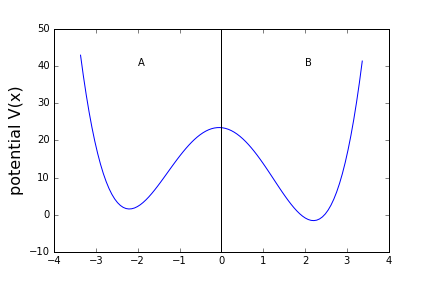
\includegraphics[width=0.6\textwidth]{Python/doublewell.png} %70% der Textbreite
	\caption{full-partition of a double-well potential}
	\label{fig:doublewell}
\end{figure}
Now compare the two model-processes $\xtilde_k$ and  $\xhat_k$.
We already know that $\xhat_k$ is a Markov chain. How about  $\xtilde_k$?
Lets investigate in possible memory effects.
For a small lag-time $\tau = 0.1$ compare the probabilities \marginpar{$\widetilde{X}$?}
\begin{equation*}
\Prob_\mu[\xtilde_{(k+1)\tau} \in A \mid \xtilde_{k\tau} \in B] \textrm{ and }
\Prob_\mu[\xtilde_{(k+1)\tau} \in A \mid \xtilde_{k\tau} \in B, \xtilde_{(k-1)\tau} \in A].
\end{equation*}
We get \marginpar{$v$ densities?}
\begin{equation}
\label{eq:recrossing1}
\Prob_\mu[\xtilde_{(k+1)\tau} \in A \mid \xtilde_{k\tau} \in B] = \int_A v_B^\tau(x) \diff x = ... ,
\end{equation}
\begin{equation}
\label{eq:recrossing2}
\Prob_\mu[\xtilde_{(k+1)\tau} \in A \mid \xtilde_{k\tau} \in B, \xtilde_{(k-1)\tau} \in A] = \int_A v_{BA}^\tau(x) \diff x = ... .
\end{equation}
So we see that for such a short lag-time $\tau$, the process $\xtilde_k$ is not memoryless and hence not a Markov process.
That effect is intuitively clear. Equation \eqref{eq:recrossing1} describes the probability to get from $B$ to $A$, so it is averaged(?) over all possible starting points in $B$. Comparing to that in \eqref{eq:recrossing2}, being in $A$ immediately one time-step before being in $B$ increases the probability that the process is still in the transition region. And to get to $A$ from the transition region in $B$ is just more likely than from any other region inside $B$.
%favorable spatial situation?

On the other hand, if we choose a large lag-time $\tau = 100$, then the past transition from $A$ to $B$ took place a long time ago. So we cannot certainly know if the process is still in the critical transition region; during that long lag-time it could also have been gone anywhere else.
%That means that we could describe the memory effect of $\xtilde$ as a \textit{short-time memory}.
That means that the memory effect included in $\xtilde$ could be called a \textit{short-time memory}.

Comparing that to $\xhat$. $\xhat$ is a Markov chain on the two possible states (=partition sets). Its transition matrix consists of the transition probabilities between these two sets within time $\tau$.
But as these probabilities are built from an originally continuous state space, they are just averaged over the whole space. That means, the probability to get from $A$ to $B$ under $\xhat$ is always the same which is not an appropriate description of the original process. In fact/for instance, being in the transition region (i.e. close to $x=0$) inside of $A$ yields a much higher probability to get into $B$ in comparison to start inside of the energy minimum of $A$. But these differences are not included in our Markov State Model.

\subsubsection*{Loss of Markov Property = Recrossing Effect} \marginpar{later = rebinding}

This loss of Markovianity of a process when projecting it onto a finite subspace is called \textit{Recrossing Effect}. \marginpar{+ proj.prop != prop.proj.?}
It is due to the fact that the projected transfer operator form in general NOT a semi-group. \marginpar{?}
%By projection onto a finite subspace we lose an important property of the transfer operator bzw generator; %namely its Markov property.
Hence, in general we have
\begin{equation*}
(P_c)^k \neq (P^k)_c.
\end{equation*}
An important question when it comes to projections of Markov processes onto lower-dimensional state spaces is shown in the following diagram.
%the time evolution of the process.
Does it make a difference if we first project the process and then propagate it and vice versa?

\begin{figure}[!ht]
	\centering
	\begin{tikzcd}
	&  \Pcal(\tau) \arrow{d}{proj.} \arrow{r}{\tau \rightarrow \tau k}    & (\Pcal(\tau))^k \arrow{d}{proj.} 			\\
	G\Pcal G \widehat{=} &  P_c (\tau)   \arrow{r}{\tau \rightarrow \tau k}            &  (P_c(\tau))^k \\
\end{tikzcd}
\caption{Projecting/propagating a transfer operator (non-commutative)}
\label{fig:diagram_transfer}
\end{figure}
%\ref{fig:diagram_transfer}
%Weber shows in habilitation that under a certain Galerkin Projection using membership functions (not    %set-based family) leads to a commuting diagram of projection and propagation. \marginpar{non-reversible?}
%+ Markov Property is preserved? \marginpar{due to proj. or trans.op.?}

%!!!
%What is the recrossing effect??? That the process loses its Markovianity? Or that there is a deviation %between project/propagate and propagate/project?

%It depends on the chosen partition of unity (the new finite-dim. state space) if the recrossing effect occurs. If %we chose a full partition for that ansatz space, then our projected process will maintain its Markovianity.
%NOP: see example above .. because xtilde != xhat

%Dieses Beispiel, in welchem das überschreiten der Barriere für
%den nächsten Zeitraum eine höhere Wahrscheinlichkeit einer erneuten
%Uberschreitung
%der Barriere bedeutet, wird auch als Recrossing Problem bezeichnet und ist in...

\subsubsection*{Discretization Error (Density Propagating Error)}
\marginpar{what about eigenv. err.?}
%However
We will present here shortly how the discretization error can be estimated in general. For our purposes that will not play an important role, since we can zurückgreifen on a transfer operator by Weber which allows a projection without(?) error.

%discretization/ projection/ propagating error
The maximal possible error between the distributions of $\widetilde{X}_k$ and $\widehat{X}_k$ after $k$ time-steps is (independently of initial distribution) given by \marginpar{which norm?}
\begin{equation*}
E(k) = \Vert G \Pcal^k G - (G \Pcal G)^k\Vert.
\end{equation*}

\begin{thm}
Assume the discrete/dominant spectrum of a transfer operator $\Pcal$ is given/denoted/ordered by $1=\lambda_0 > \lambda_1 \geq \dots \geq \lambda_n$. Then the projection error can be bounded from above in terms of the second-largest eigenvalue by
\begin{equation*}
\Vert (G \Pcal G)^k - \Pi_0\Vert \leq \Vert (G \Pcal G)^k - \Pi_0\Vert \leq \lambda_1^k,
\end{equation*}
where $\Pi_0$ is the orthogonal projection of ... .
\end{thm}

For a proof, see Sch\"utte and Sarich\cite[p.72]{schutte2013metastability}.
%illuminating
In the following chapter we will see further/deeper relations between the spectrum of the transfer operator and ... properties.
%Furthermore, there is a relation between smallness of the  projection error and the metastability of a %subdivision of the state space.
%Schuette, Huisinga. Or Sarich p.58
\marginpar{what is markov state model? def! $P_c$}
We will see how to choose partition for a MSM s.t. the approximation error becomes small. \marginpar{?}